
\chapter{The TANGO device server model}

This chapter will present the TANGO device server object model hereafter
referred as TDSOM\index{TDSOM}. First, it will introduce CORBA\index{CORBA}.
Then, it will describe each of the basic features of the TDSOM and
their function. The TDSOM can be divided into the following basic
elements - the \emph{device}, the \emph{server}, the \emph{database}
and the \emph{application programmers interface}. This chapter will
treat each of the above elements separately.


\section{Introduction to CORBA}
\label{sec:corba}

CORBA is a definition of how to write object request brokers (ORB\index{ORB}).
The definition is managed by the Object Management Group (OMG\index{OMG}
\cite{OMG-page}). Various commercial and non-commercial implementations
exist for CORBA for all the mainstream operating systems. CORBA\index{CORBA}
uses a programming language independent definition language (called
IDL) to defined network object interfaces. Language mappings are defined
from IDL\index{IDL} to the main programming languages e.g. C++, Java,
C, COBOL, Smalltalk and ADA. Within an interface, CORBA defines two
kinds of actions available to the outside world. These actions are
called \textbf{attributes\index{attribute}} and \textbf{operations}\index{operation}.

Operations are all the actions offered by an interface. For instance,
within an interface for a Thermostat class, operations could be the
action to read the temperature or to set the nominal temperature.
An attribute defines a pair of operations a client can call to send
or receive a value. For instance, the position of a motor can be defined
as an attribute because it is a data that you only set or get. A read
only attribute defines a single operation the client can call to receives
a value. In case of error, an operation is able to throw an exception
to the client, attributes cannot raises exception except system exception
(du to network fault for instance).

Intuitively, IDL interface correspond to C++ classes and IDL operations
correspond to C++ member functions and attributes as a way to read/write
public member variable. Nevertheless, IDL defines only the interface
to an object and say nothing about the object implementation. IDL
is only a descriptive language. Once the interface is fully described
in the IDL language, a compiler (from IDL to C++, from IDL to Java...)
generates code to implement this interface. Obviously, you still have
to write how operations are implemented.

The act of invoking an operation on an interface causes the ORB to
send a message to the corresponding object implementation. If the
target object is in another address space, the ORB run time sends
a remote procedure call to the implementation. If the target object
is in the same address space as the caller, the invocation is accomplished
as an ordinary function call to avoid the overhead of using a networking
protocol.

For an excellent reference on CORBA\index{CORBA} with C++ refer to
\cite{Henning}. The complete TANGO IDL\index{IDL} file can be found
in the TANGO web page\cite{Tango web} or at the end of this document
in the appendix 2 chapter.


\section{The model}

The basic idea of the TDSOM\index{TDSOM} is to treat each device
as an \textbf{object}. Each device is a separate entity which has
its own data and behavior. Each device has a unique name which identifies
it in network name space. Devices are organized according to \textbf{classes},
each device belonging to a class. All classes are derived from one
root class thus allowing some common behavior for all devices. Four
kind of requests can be sent to a device (locally i.e. in the same
process, or remotely i.e. across the network) :
\begin{itemize}
\item Execute actions via \textbf{commands\index{command}}
\item Read/Set data specific to each device belonging to a class via TANGO
\textbf{attributes\index{attribute}}
\item Read/Set data specific to each device belonging to a class via TANGO
\textbf{pipes}\index{pipe}
\item Read some basic device data available for all devices via CORBA attributes.
\item Execute a predefined set of actions available for every devices via
CORBA operations\index{operation}
\end{itemize}
Each device is stored in a process called a \textbf{device server}\index{server}.
Devices are configured at runtime via \textbf{properties\index{properties}}
which are stored in a \textbf{database}\index{database}.


\section{The device}
\label{sec:dev}

The device is the heart of the TDSOM. A device is an abstract concept
defined by the TDSOM. In reality, it can be a piece of hardware (an
interlock bit) a collection of hardware (a screen attached to a stepper
motor) a logical device (a taper) or a combination of all these (an
accelerator). Each device has a unique name in the control system
and eventually one alias\index{alias}. Within Tango, a four field
name\index{name} space has been adopted consisting of \begin{center}{[}//FACILITY/{]}DOMAIN/CLASS/MEMBER\end{center}
Facility refers to the control system instance, domain refers to the
sub-system, class the class and member the instance of the device.
Device name alias(es) must also be unique within a control system.
There is no predefined syntax for device name alias.

Each device belongs to a class. The device class contains a complete
description and implementation of the behavior of all members of that
class. New device classes can be constructed out of existing device
classes. This way a new hierarchy of classes can be built up in a
short time. Device classes can use existing devices as sub-classes
or as sub-objects. The practice of reusing existing classes is classical
for Object Oriented Programming and is one of its main advantages.

All device classes are derived from the same class (the device root
class) and implement \textbf{the same CORBA interface}. All devices
implementing the same CORBA interface ensures all control object support
the same set of CORBA operations and attributes. The device root class
contains part of the common device code. By inheriting from this class,
all devices shared a common behavior. This also makes maintenance
and improvements to the TDSOM easy to carry out.

All devices also support a \textbf{black box\index{black-box}} where
client requests for attributes or operations are recorded. This feature
allows easier debugging session for device already installed in a
running control system.


\subsection{The commands\index{command}}

Each device class implements a list of commands. Commands are very
important because they are the client's major dials and knobs for
controlling a device. Commands have a fixed calling syntax - consisting
of one input argument and one output argument. Arguments type must
be chosen in a fixed set of data types: All simple types (boolean,
short, long (32 bits), long (64 bits), float, double, unsigned short,
unsigned long (32 bits), unsigned long (64 bits) and string) and arrays
of simple types plus array of strings and longs and array of strings
and doubles). Commands can execute any sequence of actions. Commands
can be executed synchronously (the requester is blocked until the
command ended) or asynchronously (the requester send the request and
is called back when the command ended).

Commands are executed using two CORBA operations named \textbf{command\_inout\index{command-inout}}
for synchronous commands and \textbf{command\_inout\_async\index{command-inout-async}}
for asynchronous commands. These two operations called a special method
implemented in the device root class - the \emph{command\_handler\index{command-handler}}
method. The \emph{command\_handler} calls an \emph{is\_allowed\index{is-allowed}}
method implemented in the device class before calling the command
itself. The \emph{is\_allowed} method is specific to each command%
\footnote{In contrary to the state\_handler method of the TACO device server
model which is not specific to each command.%
}. It checks to see whether the command to be executed is compatible
with the present device state. The command function is executed only
if the \emph{is\_allowed} method allows it. Otherwise, an exception
is sent to the client.


\subsection{The TANGO attributes\index{attribute}}

In addition to commands, TANGO devices also support normalized data
types called attributes%
\footnote{TANGO attributes were known as signals in the TACO device server model%
}. Commands are device specific and the data they transport are not
normalized i.e. they can be any one of the TANGO data types with no
restriction on what each byte means. This means that it is difficult
to interpret the output of a command\index{command} in terms of what
kind of value(s) it represents. Generic display programs need to know
what the data returned represents, in what units it is, plus additional
information like minimum, maximum, quality etc. Tango attributes solve
this problem.

TANGO attributes are zero, one or two dimensional data which have
a fix set of properties e.g. quality, minimum and maximum, alarm low
and high. They are transferred in a specialized TANGO type and can
be read, write or read-write. A device can support a list of attributes.
Clients can read one or more attributes from one or more devices.
To read TANGO attributes, the client uses the \textbf{read\_attributes\index{read-attributes}}
operation. To write TANGO attributes, a client uses the \textbf{write\_attributes\index{write-attributes}}
operation. To write then read TANGO attributes within the same network
request, the client uses the \textbf{write\_read\_attributes\index{write-read-attribute}}
operation. To query a device for all the attributes it supports, a
client uses the \textbf{get\_attribute\_config\index{get-attribute-config}}
operation. A client is also able to modify some of parameters defining
an attribute with the \textbf{set\_attribute\_config\index{set-attribute-config}}
operation. These five operations are defined in the device CORBA interface.

TANGO support thirteen data types for attributes (and arrays of for
one or two dimensional data) which are: boolean, short, long (32 bits),
long (64 bits), float, double, unsigned char, unsigned short, unsigned
long (32 bits), unsigned long (64 bits), string, a specific data type
for Tango device state and finally another specific data type to transfer
data as an array of unsigned char with a string describing the coding
of these data.


\subsection{The TANGO pipes\index{pipe}}

Since release 9, in addition to commands and attributes, TANGO devices
also support pipes.

In some cases, it is required to exchange data between client and
device of varrying data type. This is for instance the case of data
gathered during a scan on one experiment. Because the number of actuators
and sensors involved in the scan may change from one scan to another,
it is not possible to use a well defined data type. TANGO pipes have
been designed for such cases. A TANGO pipe is basically a pipe dedicated
to transfer data between client and device. A pipe has a set of two
properties which are the pipe label and its description. A pipe can
be read or read-write. A device can support a list of pipes. Clients
can read one or more pipes from one or more devices. To read a TANGO
pipe, the client uses the \textbf{read\_pipe\index{read-pipe}} operation.
To write a TANGO pipe, a client uses the \textbf{write\_pipe\index{write-pipe}}
operation. To write then read a TANGO pipe within the same network
request, the client uses the \textbf{write\_read\_pipe\index{write-read-pipe}}
operation. To query a device for all the pipes it supports, a client
uses the \textbf{get\_pipe\_config\index{get-pipe-config}} operation.
A client is also able to modify some of parameters defining a pipe
with the \textbf{set\_pipe\_config\index{set-pipe-config}} operation.
These five operations are defined in the device CORBA interface.

In contrary of commands or attributes, a TANGO pipe does not have
a pre-defined data type. Data transferred through pipes may be of
any basic Tango data type (or array of) and this may change every
time a pipe is read or written. 


\subsection{Command, attributes or pipes ?}

There are no strict rules concerning what should be returned as command
result and what should be implemented as an attribute or as a pipe.
Nevertheless, attributes are more adapted to return physical value
which have a kind of time consistency. Attribute also have more properties
which help the client to precisely know what it represents. For instance,
the state and the status of a power supply are not physical values
and are returned as command result. The current generated by the power
supply is a physical value and is implemented as an attribute. The
attribute properties allow a client to know its unit, its label and
some other informations which are related to a physical value. Command
are well adapted to send order to a device like switching from one
mode of operation to another mode of operation. For a power supply,
the switch from a STANDBY mode to a ON mode is typically done via
a command. Finally pipe is well adapted when the kind and number of
data exchanged between the client and the device change with time.


\subsection{The CORBA attributes}

Some key data implemented for each device can be read without the
need to call a command or read an attribute. These data are :
\begin{itemize}
\item The device state\index{state}
\item The device status\index{status}
\item The device name\index{name}
\item The administration device name called adm\_name\index{administration}
\item The device description\index{description}
\end{itemize}
The device state is a number representing its state. A set of predefined
states are defined in the TDSOM. The device status is a string describing
in plain text the device state and any additional useful information
of the device as a formatted ascii string. The device name is its
name as defined in \ref{sec:dev}. For each set of devices grouped
within the same server, an administration device is automatically
added. This adm\_name is the name of the administration device. The
device description is also an ascii string describing the device rule.

These five CORBA attributes are implemented in the device root class
and therefore do not need any coding from the device class programmer.
As explained in \ref{sec:corba}, the CORBA attributes are not allowed
to raise exceptions whereas command (which are implemented using CORBA
operations) can.


\subsection{The remaining CORBA operations}

The TDSOM also supports a list of actions defined as CORBA operations
in the device interface and implemented in the device root class.
Therefore, these actions are implemented automatically for every TANGO
device. These operations are :
\begin{lyxlist}{MMMMMMMMMMM}
\item [{ping\index{ping}}] to ping a device to check if the device is
alive. Obviously, it checks only the connection from a client to the
device and not all the device functionalities
\item [{command\_list\_query\index{command-list-query}}] request a list
of all the commands supported by a device with their input and output
types and description
\item [{command\_query\index{command-query}}] request information about
a specific command which are its input and output type and description
\item [{info\index{info}}] request general information on the device like
its name, the host where the device server hosting the device is running...
\item [{black\_box\index{black-box}}] read the device black-box as an
array of strings
\end{lyxlist}

\subsection{The special case of the device state and status}

Device state\index{state} and status\index{status} are the most
important key device informations. Nearly all client software dealing
with Tango device needs device(s) state and/or status. In order to
simplify client software developper work, it is possible to get these
two piece of information in three different manners :
\begin{enumerate}
\item Using the appropriate CORBA attribute (state or status)
\item Using command on the device. The command are called State or Status
\item Using attribute. Even if the state and status are not real attribute,
it is possible to get their value using the read\_attributes operation.
Nevertheless, it is not possible to set the attribute configuration
for state and status. An error is reported by the server if a client
try to do so.
\end{enumerate}

\subsection{The device polling\index{polling}}

Within the Tango framework, it is also possible to force executing
command(s) or reading attribute(s) at a fixed frequency. It is called
\emph{device polling}. This is automatically handled by Tango core
software with a polling threads pool. The command result or attribute
value are stored in circular buffers. When a client want to read attribute
value (or command result) for a polled attribute (or a polled command),
he has the choice to get the attribute value (or command result) with
a real access to the device of from the last value stored in the device
ring buffer. This is a great advantage for ``slow'' devices. Getting
data from the buffer is much faster than accessing the device itself.
The technical disadvantage is the time shift between the data returned
from the polling buffer and the time of the request. Polling a command
is only possible for command without input arguments. It is not possible
to poll a device pipe\index{pipe}.

Two other CORBA operations called \emph{command\_inout\_history\_X\index{command-inout-history-X}}
and \emph{read\_attribute \_history\_X\index{read-attribute-history-X}}
allow a client to retrieve the history of polled command or attribute
stored in the polling buffers. Obviously, this history is limited
to the depth of the polling buffer. 

The whole polling system is available only since Tango release 2.x
and above in CPP and since TangORB release 3.7.x and above in Java.


\section{The server}

Another integral part of the TDSOM is the server concept. The server
(also referred as device server\index{server}) is a process whose
main task is to offer one or more services to one or more clients.
To do this, the server has to spend most of its time in a wait loop
waiting for clients to connect to it. The devices are hosted in the
server process. A server is able to host several classes of devices.
In the TDSOM, a device of the \textbf{DServer} class is automatically
hosted by each device server. This class of device supports commands
which enable remote device server process administration.

TANGO supports device server process on two families of operating
system : Linux and Windows.


\section{The Tango Logging\index{logging} Service}
\label{sec:The-Tango-Logging}

During software life, it is always convenient to print miscellaneous
informations which help to:
\begin{itemize}
\item Debug the software
\item Report on error
\item Give regular information to user
\end{itemize}
This is classically done using cout (or C printf) in C++ or println
method in Java language. In a highly distributed control system, it
is difficult to get all these informations coming from a high number
of different processes running on a large number of computers. Since
its release 3, Tango has incorporated a Logging Service called the
Tango Logging Service (TLS) which allows print messages to be:
\begin{itemize}
\item Displayed on a console (the classical way)
\item Sent to a file
\item Sent to specific Tango device called log consumer\index{consumer}.
Tango package has an implementation of log consumer where every consumer
device is associated to a graphical interface. This graphical interface
display messages but could also be used to sort messages, to filter
messages... Using this feature, it is possible to centralise display
of these messages coming from different devices embedded within different
processes. These log consumers can be:

\begin{itemize}
\item Statically configured meaning that it memorizes the list of Tango
devices for which it will get and display messages.
\item Dynamically configured. The user, with the help of the graphical interface,
chooses devices from which he want to see messages.
\end{itemize}
\end{itemize}

\section{The database\index{database}}

To achieve complete device independence, it is necessary however to
supplement device classes with a possibility for configuring device
dependencies at runtime. The utility which does this in the TDSOM
is the \textbf{property database}. Properties%
\footnote{Properties were known as resources in the TACO device server model%
} are identified by an ascii string and the device name. TANGO attributes\index{attribute}
are also configured using properties\index{properties}. This database
is also used to store device network addresses (CORBA IOR\index{IOR}'s),
list of classes hosted by a device server process and list of devices
for each class in a device server process. The database ensure the
uniqueness of device name and of alias. It also links device name
and it list of aliases.

TANGO uses MySQL\index{MySQL}\cite{mysql} as its database. MySQL
is a relational database which implements the SQL language. However,
this is largely enough to implement all the functionalities needed
by the TDSOM. The database is accessed via a classical TANGO device
hosted in a device server. Therefore, client access the database via
TANGO commands requested on the database device. For a good reference
on MySQL refer to \cite{MySQL book}


\section{The controlled access}

Tango also provides a controlled access\index{controlled-access}
system. It's a simple controlled access system. It does not provide
encrypted communication or sophisticated authentification. It simply
defines which user (based on computer loggin authentification) is
allowed to do which command (or write attribute) on which device and
from which host. The information used to configure this controlled
access feature are stored in the Tango database and accessed by a
specific Tango device server which is not the classsical Tango database
device server described in the previous section. Two access levels
are defined:
\begin{itemize}
\item Everything is allowed for this user from this host
\item The write-like calls on the device are forbidden and according to
configuration, a command subset is also forbidden for this user from
this host
\end{itemize}
This feature is precisely described in the chapter \textquotedbl{}Advanced
features\textquotedbl{}


\section{The Application Programmers Interfaces}


\subsection{Rules of the API}

While it is true TANGO clients can be programmed using only the CORBA
API, CORBA knows nothing about TANGO. This means client have to know
all the details of retrieving IORs from the TANGO database, additional
information to send on the wire, TANGO version control etc. These
details can and should be wrapped in TANGO Application Programmer
Interface (API). The API is implemented as a library in C++ and as
a package in Java. The API is what makes TANGO clients easy to write.
The API's consists the following basic classes :
\begin{itemize}
\item DeviceProxy which is a \emph{proxy} to the real device
\item DeviceData to encapsulate data send/receive from/to device via commands
\item DeviceAttribute to encapsulate data send/receive from/to device via
attributes
\item Group which is a \emph{proxy} to a group\index{group} of devices
\end{itemize}
In addition to these main classes, many other classes allows a full
interface to TANGO features. The following figure is a drawing of
a typical client/server application using TANGO.

\vspace{0.3cm}


\begin{center}
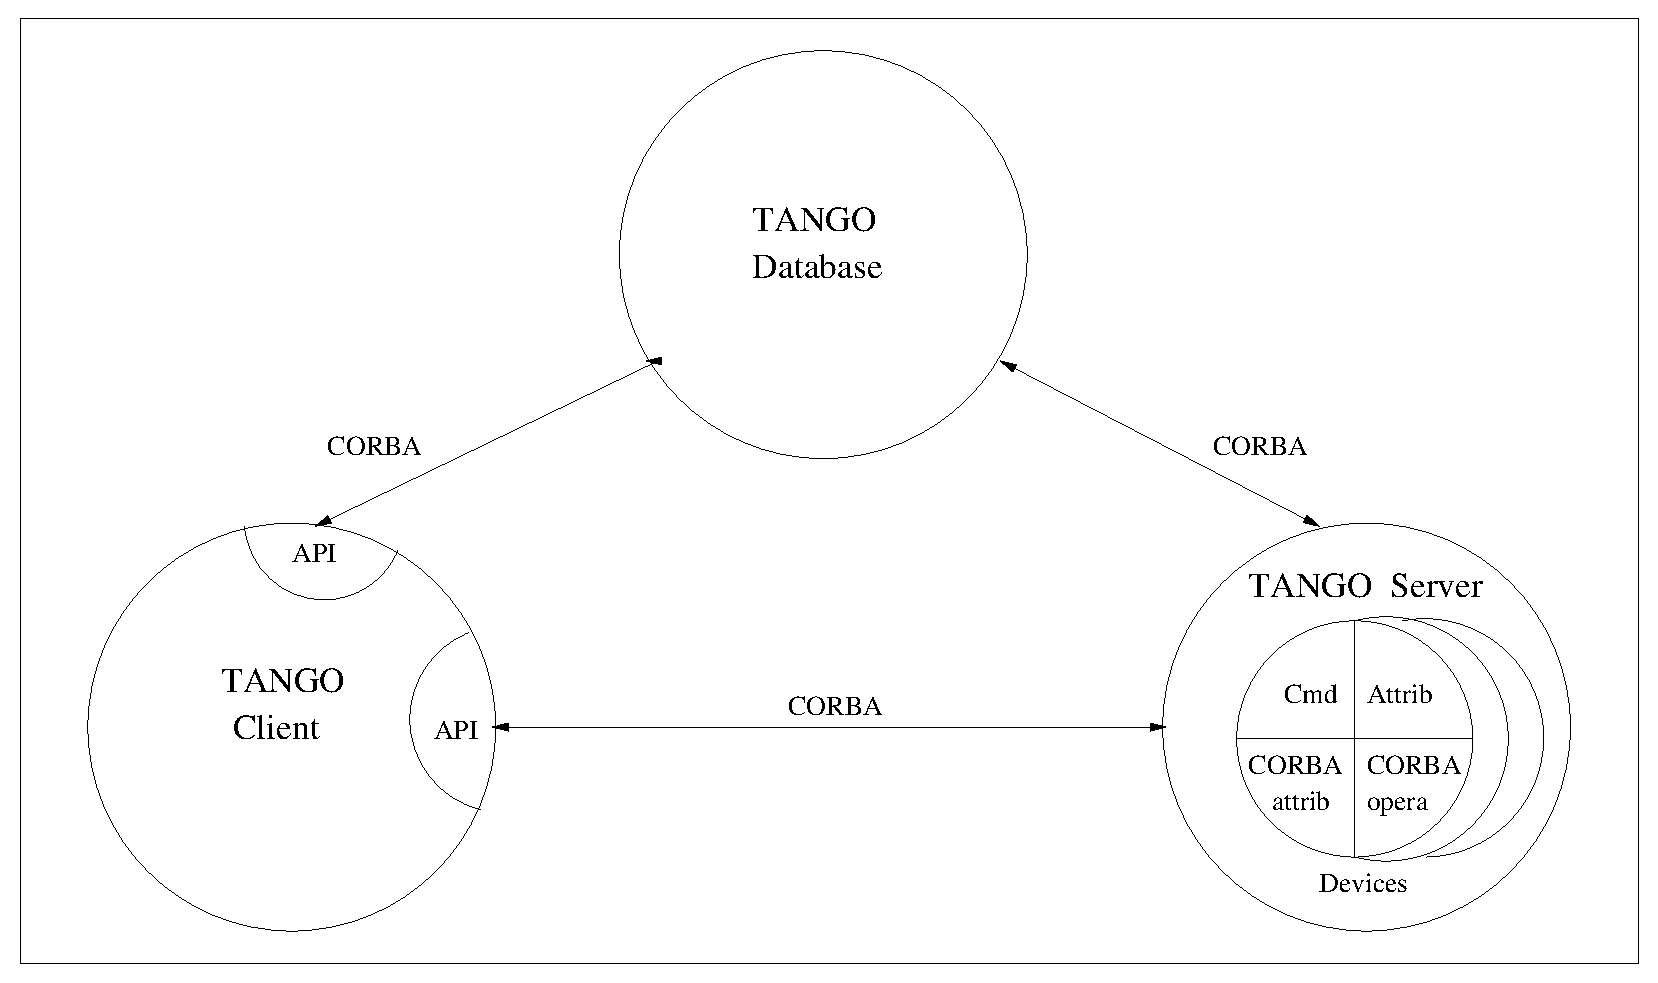
\includegraphics[width=12cm,height=7cm]{ds_model/archi}
\par\end{center}

\vspace{0.3cm}


The database is used during server and client startup phase to establish
connection between client and server.


\subsection{Communication between client and server using the API}

With the API, it is possible to request command to be executed on
a device or to read/write device attribute(s) using one of the two
communication models implemented. These two models are:
\begin{enumerate}
\item The synchronous model where client waits (and is blocked) for the
server to send the answer or until the timeout is reached
\item The asynchronous model. In this model, the clients send the request
and immediately returns. It is not blocked. It is free to do whatever
it has to do like updating a graphical user interface. The client
has the choice to retrieve the server answer by checking if the reply
is arrived by calling an API specific call or by requesting that a
call-back method is executed when the client receives the server answer.
\end{enumerate}
The asynchronous model is available with Tango release 3 and above.


\subsection{Tango events}

On top of the two communication model previously described, TANGO
offers an \textquotedbl{}event system\textquotedbl{}\index{event}.
The standard TANGO communication paradigm is a synchronou/asynchronous
two-way call. In this paradigm the call is initiated by the client
who contacts the server. The server handles the client's request and
sends the answer to the client or throws an exception which the client
catches. This paradigm involves two calls to receive a single answer
and requires the client to be active in initiating the request. If
the client has a permanent interest in a value he is obliged to poll
the server for an update in a value every time. This is not efficient
in terms of network bandwidth nor in terms of client programming.

For clients who are permanently interested in values the event-driven
communication paradigm is a more efficient and natural way of programming.
In this paradigm the client registers his interest once in an event
(value). After that the server informs the client every time the event
has occurred. This paradigm avoids the client polling, frees it for
doing other things, is fast and makes efficient use of the network.

Before TANGO release 8, TANGO used the CORBA OMG COS Notification
Service\index{Notification Service} to generates events. TANGO uses
the omniNotify\index{omniNotify} implementation of the Notification
service. omniNotify was developed in conjunction with the omniORB
CORBA implementation also used by TANGO. The heart of the Notification
Service is the notification daemon. The omniNotify daemons are the
processes which receive events from device servers and distribute
them to all clients which are subscribed. In order to distribute the
load of the events there is one notification daemon per host. Servers
send their events to the daemon on the local host. Clients and servers
get the IOR for the host from the TANGO database. 

The following figure is a schematic of the Tango event system for
Tango releases before Tango 8.

\vspace{0.3cm}


\begin{center}
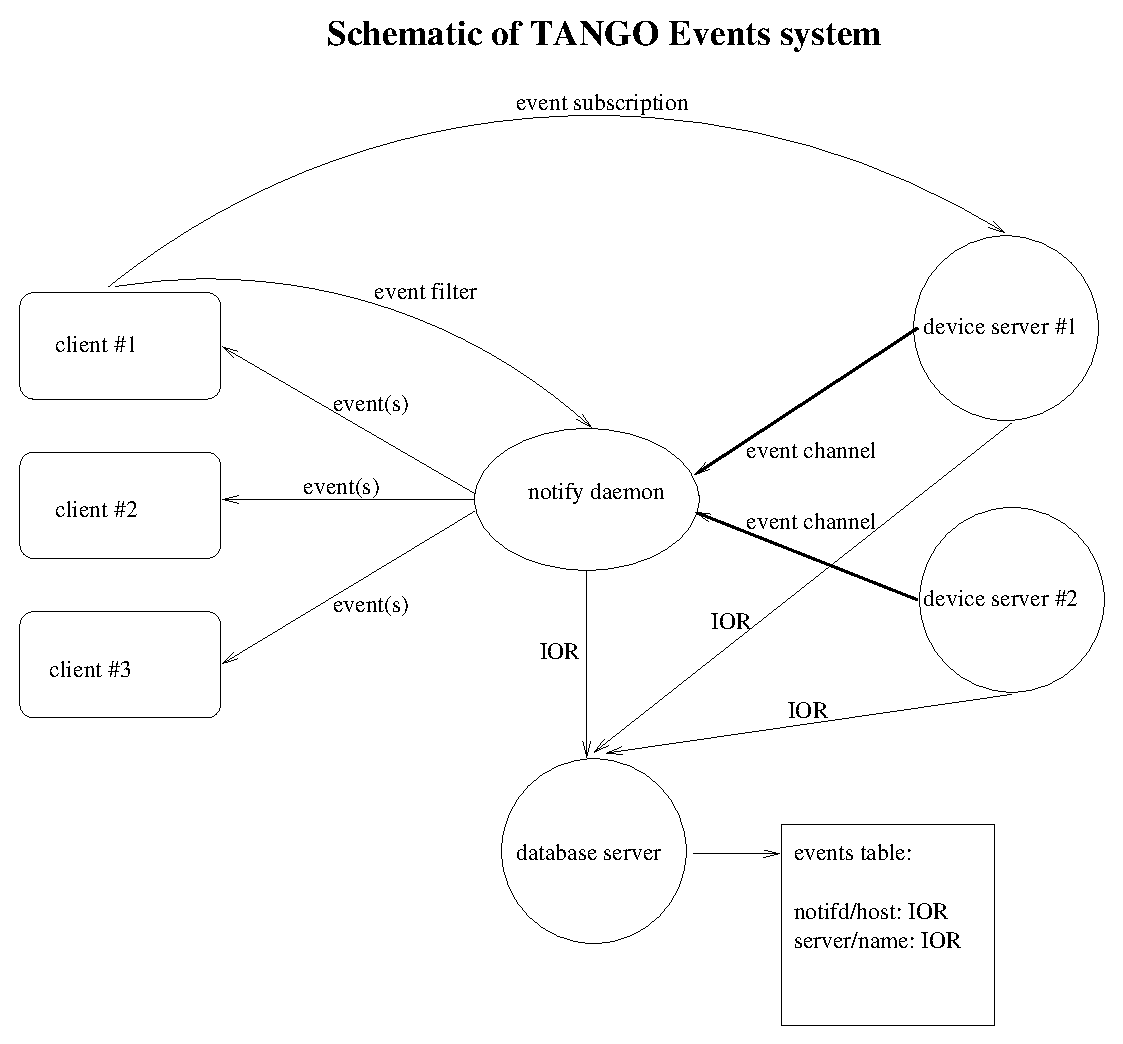
\includegraphics[bb=0bp 0bp 523bp 485bp,clip,scale=0.8]{ds_model/event_schematic}
\par\end{center}

\vspace{0.3cm}


Starting with Tango 8, a new design of the event system has been implemented.
This new design is based on the ZMQ\index{ZMQ} library. ZMQ is a
library allowing users to create communicating system. It implements
several well known communication pattern including the Publish/Subscribe\index{Publish/Subscribe}
pattern which is the basic of the new Tango event system. Using this
library, a separate notification service is not needed anymore and
event communiction is available with only client and server processes
which simplifies the overall design. Starting with Tango 8.1, the
event propagation between devices and clients could be done using
a multicasting\index{multicasting} protocol. The aim of this is to
reduce both the network bandwidth use and the CPU consumption on the
device server side. See chapter on Advanced Features to get all the
details on this feature.

The following figure is a schematic of the Tango event system for
Tango releases starting with Tango release 8.

\vspace{0.3cm}


\begin{center}
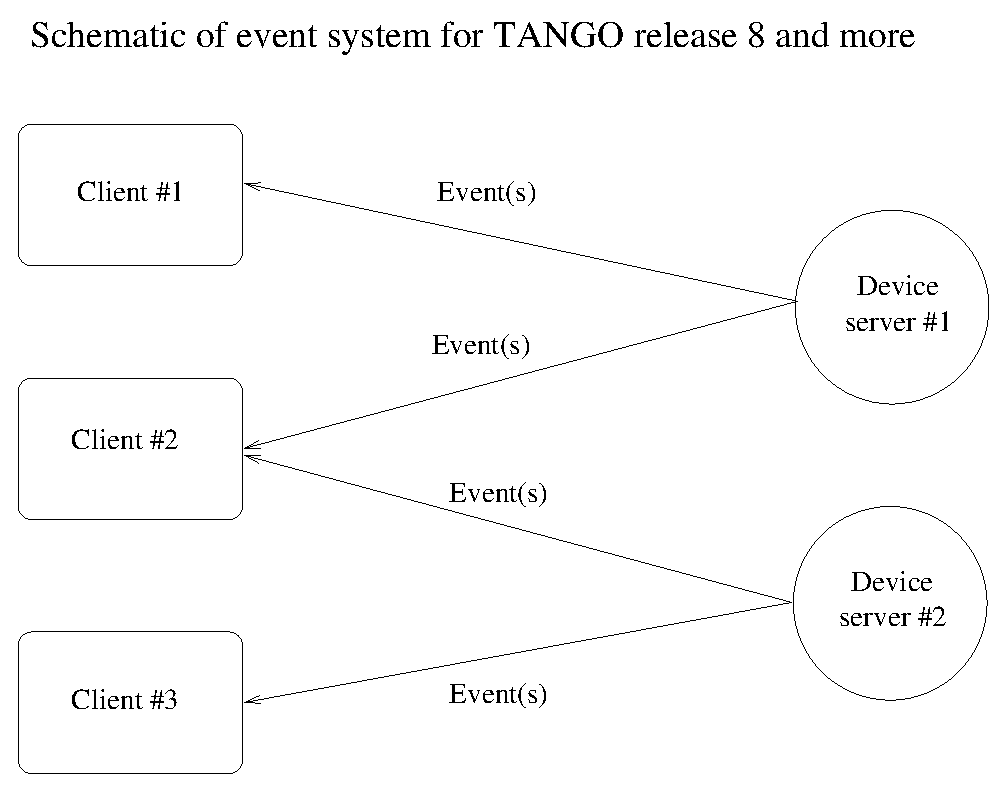
\includegraphics[bb=0bp 0bp 523bp 485bp,clip,scale=0.8]{ds_model/event_schematic_zmq}
\par\end{center}

\vspace{0.3cm}


\begin{center}

\vspace{5cm}


\label{OneRicardo}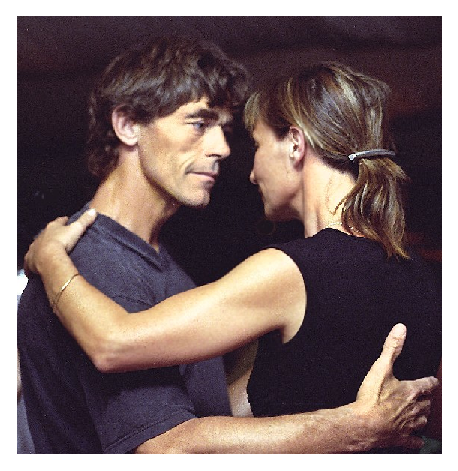
\includegraphics[scale=1.5]{dance/Eltaita-reduc}

\end{center}
